\documentclass[20pt,a4paper]{extarticle}
\usepackage[utf8]{inputenc}
\usepackage[english]{babel}

\usepackage{amsmath}
\usepackage{amsfonts}
\usepackage{amssymb}
\usepackage{mathtools}
\usepackage{systeme}
\sysdelim..

\usepackage{graphicx}
\usepackage{caption}
\usepackage{subcaption}
\usepackage{lmodern}
\usepackage{tikz}
\usetikzlibrary{calc}
\usepackage{titlesec}
\usepackage{environ}
\usepackage{xcolor}
\usepackage{fancyhdr}
\usepackage[colorlinks = true, linkcolor = black]{hyperref}
\usepackage{xparse}
\usepackage{enumitem}
\usepackage{comment}
\usepackage{wrapfig}
\usepackage{soul}
\usepackage[capitalise]{cleveref}

\usepackage[left=1cm,right=1cm,top=1cm,bottom=3cm]{geometry}
\usepackage{multicol}
\usepackage[indent=0pt]{parskip}

\newcommand{\spaceP}{\vspace*{0.5cm}}
\newcommand{\Span}{\mathrm{Span}\,}
\newcommand{\range}{\mathrm{range}\,}
\newcommand{\ra}{\rightarrow}
\newcommand{\curl}{\mathrm{curl} \,}
\newcommand{\hint}[1]{\scalebox{2}{$\displaystyle\int_{\scalebox{0.35}{$#1$}}$}\,}
\newcommand{\hiint}[1]{\scalebox{2}{$\displaystyle\iint_{\scalebox{0.35}{$#1$}}$}\,}
\newcommand{\hiiint}[1]{\scalebox{2}{$\displaystyle\iiint_{\scalebox{0.35}{$#1$}}$}\,}
\renewcommand{\div}{\mathrm{div}\,}

\makeatletter
\renewcommand*\env@matrix[1][*\c@MaxMatrixCols c]{%
  \hskip -\arraycolsep
  \let\@ifnextchar\new@ifnextchar
  \array{#1}}
\makeatother

%% Redefining sections
\newcommand{\sectionformat}[1]{%
    \begin{tikzpicture}[baseline=(title.base)]
        \node[rectangle, draw] (title) {#1};
    \end{tikzpicture}
    
    \noindent\hrulefill
}

\newif\ifhNotes 

\hNotesfalse

\ifhNotes
	\newcommand{\hideNotes}[1]{%
	\phantom{#1}
	}
	\newcommand{\hideNotesU}[1]{%
	\underline{\hspace{1mm}\phantom{#1}\hspace{1mm}}
	}
\else
	\newcommand{\hideNotes}[1]{#1}
	\newcommand{\hideNotesU}[1]{\textcolor{blue}{#1}}
\fi

% default values copied from titlesec documentation page 23
% parameters of \titleformat command are explained on page 4
\titleformat%
    {\section}% <command> is the sectioning command to be redefined, i. e., \part, \chapter, \section, \subsection, \subsubsection, \paragraph or \subparagraph.
    {\normalfont\large\scshape}% <format>
    {}% <label> the number
    {0em}% <sep> length. horizontal separation between label and title body
    {\centering\sectionformat}% code preceding the title body  (title body is taken as argument)

%% Set counters for sections to none
\setcounter{secnumdepth}{0}

%% Set the footer/headers
\pagestyle{fancy}
\fancyhf{}
\renewcommand{\headrulewidth}{0pt}
\renewcommand{\footrulewidth}{2pt}
\lfoot{P.-O. Paris{\'e}}
\cfoot{MATH 311}
\rfoot{Page \thepage}

%% Defining example environment
\newcounter{example}
\NewEnviron{example}%
	{%
	\noindent\refstepcounter{example}\fcolorbox{gray!40}{gray!40}{\textsc{\textcolor{red}{Example~\theexample.}}}%
	%\fcolorbox{black}{white}%
		{  %\parbox{0.95\textwidth}%
			{
			\BODY
			}%
		}%
	}

\newcounter{theorem}
\NewEnviron{theorem}%
	{%
	\noindent\refstepcounter{theorem}\fcolorbox{gray!40}{gray!40}{\textsc{\textcolor{black}{Theorem~\thetheorem.}}}%
	%\fcolorbox{black}{white}%
		{  %\parbox{0.95\textwidth}%
			{
			\BODY
			}%
		}%
	}

\newcounter{definition}
\NewEnviron{definition}%
	{%
	\noindent\refstepcounter{definition}\fcolorbox{gray!40}{gray!40}{\textsc{\textcolor{black}{Definition~\thedefinition.}}}%
	%\fcolorbox{black}{white}%
		{  %\parbox{0.95\textwidth}%
			{
			\BODY
			}%
		}%
	}

\newcounter{algo}
\NewEnviron{algorithm}
	{%
	\noindent\refstepcounter{algo}\fcolorbox{gray!40}{gray!40}{\textsc{\textcolor{black}{Algorithm~\thealgo.}}}%
	%\fcolorbox{black}{white}%
		{  %\parbox{0.95\textwidth}%
			{
			\BODY
			}%
		}%
	}

\NewEnviron{solution}%
	{%
	\noindent \fcolorbox{gray!40}{gray!40}{\textsc{\textcolor{blue}{Solution.}}}%
	%\fcolorbox{black}{white}%
		{  %\parbox{0.95\textwidth}%
			{
			%\textcolor{blue}
			}%
		}%
	}

\NewEnviron{proof}%
	{%
	\noindent \fcolorbox{gray!40}{gray!40}{\textsc{\textcolor{blue}{Proof.}}}%
	%\fcolorbox{black}{white}%
		{  %\parbox{0.95\textwidth}%
			{
			\textcolor{blue}{%
			\BODY
			}
			}%
		}%
	}
%%% Ignorer les notes
%\excludecomment{notes}

%%%%
\begin{document}
\thispagestyle{empty}

\begin{center}
\vspace*{2.5cm}

{\Huge \textsc{Math 311}}

\vspace*{1.5cm}

{\LARGE \textsc{Chapter 2}} 

\vspace*{0.75cm}

\noindent\textsc{Section 2.5: Elementary Matrices}

\vspace*{0.75cm}

\tableofcontents

\vfill

\noindent \textsc{Created by: Pierre-Olivier Paris{\'e}} \\
\textsc{Spring 2024}
\end{center}

\newpage

\section{Basics}

\begin{example}
Let $E_1 = \begin{bmatrix} 0 & 1 \\ 1 & 0 \end{bmatrix}$, $E_2 = \begin{bmatrix} 1 & 0 \\ 0 & 9 \end{bmatrix}$, and $E_3 = \begin{bmatrix} 1 & 5 \\ 0 & 1 \end{bmatrix}$. Let $A = \begin{bmatrix} 3 & 2 & 1 \\ 1 & 2 & 3 \end{bmatrix}$.
	\begin{enumerate}[label=\alph*)]
		\item Find $E_1 A$ and interprete the result.
		\item Find $E_2 A$ and interprete the result.
		\item Find $E_3 A$ and interprete the result.
	\end{enumerate}
\end{example}

\begin{solution}

\end{solution}

\newpage 

\begin{definition}
An $n \times n$ matrix $E$ is called an \textbf{elementary matrix} if it can be obtained from the identity matrix $I_n$ by a single elementary row operation. We say that $E$ is of type I, II, or III if the operation used to obtain $E$ is of that type.
\end{definition}

\begin{theorem}
\begin{enumerate}
	\item If an elementary row operation is performed on an $m \times n$ matrix $A$, then the result is $EA$, where $E$ is the associated elementary matrix.
	\item Every elementary matrix $E$ is invertible, and $E^{-1}$ correspond to the inverse of the row operation that produces $E$.
\end{enumerate}
\end{theorem}

\underline{Reminder:}
	\begin{center}
	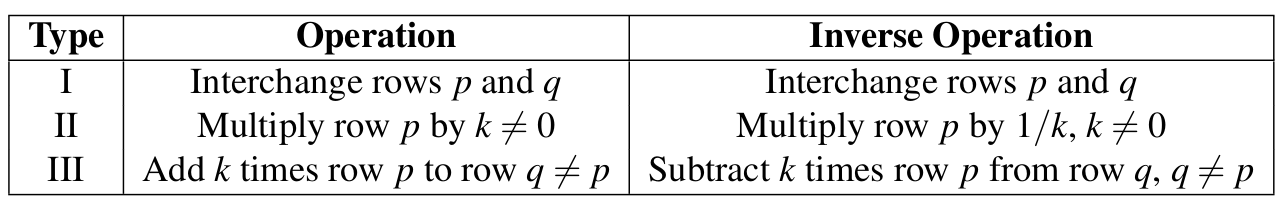
\includegraphics[scale=0.4]{table-reminder.png}
	\end{center}

\begin{example}
For each of the following matrices, describe the corresponding row operation and write the inverse.
	\[
		E_1 = \begin{bmatrix} 
		1 & 0 & 3 \\ 0 & 1 & 0 \\ 0 & 0 & 1 \end{bmatrix} \quad \text{ and } \quad E_2 = \begin{bmatrix} 0 & 1 & 0 \\ 1 & 0 & 0 \\ 0 & 0 & 1 \end{bmatrix} .
	\]
\end{example}

\newpage 

\section{Inverses and Elementary Matrices}

\begin{example}
By recording each row operation as an elementary matrix, show that the invertible matrix $A = \begin{bmatrix} 1 & 1 \\ 2 & 1 \end{bmatrix}$ is a product of elementary matrices.
\end{example}

\begin{solution}

\end{solution}

\vfill 

\begin{theorem}
A square matrix is invertible if and only if it is a product of elementary matrices.
\end{theorem}

\newpage 

Assume that an $m \times n$ matrix $A$ is carried to a matrix $B$ (written $A \ra B$) by a series of $k$ elementary row operations.

Let $E_1$, $E_2$, $\ldots$, $E_k$ be the corresponding elementary matrices. Then
	\[
		A I_m \ra E_1 A \ra E_2 E_1 A \ra \cdots \ra E_k E_{k-1} \cdots E_2 E_1 A = B .
	\]

Writing $U = E_k E_{k-1} \cdots E_2 E_1$, then $U$ is invertible and $B = UA$.

\begin{definition}
We say that two matrices $A$ and $B$ are \textbf{row-equivalent} if there is an invertible matrix $U$ such that $B = UA$.
\end{definition}

\begin{example}
Express the RREF of the matrix $A = \begin{bmatrix} 1 & -1 & 2 \\ -2 & 1 & 0\end{bmatrix}$ and a product $UA$, with $U$ a $2 \times 2$ invertible matrix.
\end{example}

\begin{solution}

\end{solution}

\end{document}